
\section*{Attacks}
\subsection*{Attacks in the context model}
\begin{frame}{Attacks in the context model}

\resizebox{!}{0.6\textwidth}
{
\tikzstyle{man}=[font={\Gentsroom}, scale=5]
\tikzstyle{woman}=[font={\Ladiesroom}, scale=5]

\begin{tikzpicture}[every node/.style={inner sep=0,outer sep=0}, arrows={[round]}]

\draw (-5.5,6) rectangle (2,-0.5);
\node at (-1,5.5) {Household};

\draw  (-6.5,7) [fill=white] rectangle (-4,5.5) node[pos=.5,align=center] {Home\\Production};
\draw  (-5,1.5) [fill=white] rectangle (-3.5,0) node[pos=.5,align=center] {Smart\\Meter};
\draw  (-3,4.5) [fill=white] rectangle (-1,3) node[pos=.5,align=center] {Smart\\Appliance};
\draw  (-0.5,2) [fill=white] rectangle (0.5,1) node[pos=.5,align=center] {Client};
\draw  (-9,2.5) [fill=white] rectangle (-6.5,1) node[pos=.5,align=center] {Data Hub};

\node[man] (consumer) at (1,1) {};
\node [below=0.2 of consumer] {Consumer};

\node[man] (burglar) at (-6.5,0) {};
\node [below=0.2 of burglar] {Burglar};

\node[man] (external) at (3.5,5) {};
\node [below=0.2 of external] {External};

\node[man] (power) at (-7.5,6.5) {};
\node [below=0.2 of power,align=center] {Electrical\\Company};

\node[man] (distribution) at (-7.5,4) {};
\node [below=0.2 of distribution] {Distribution};

\node[woman] (partner) at (1,4) {};
\node [below=0.2 of partner] {Partner};

\node[man] (neighbor) at (3.5,0.5) {};
\node [below=0.2 of neighbor] {Neighbor};

\draw[dashed] (-4.5,5.5) -- (-4.5,1.5);
\draw[dashed] (-6.5,1.5) -- (-6,1.5) -- (-6,1) -- (-5,1);
\draw[dashed] (-3.5,1) -- (-2.5,1) -- (-2.5,1.5) -- (-0.5,1.5);
\draw[dashed] (-2.5,3) -- (-2.5,2.25) -- (-4,2.25) -- (-4,1.5);

\draw[ultra thick, red, -{Stealth[scale=1.2]}, bend right=90] (power) to[out=-10,in=190] (consumer);
\draw[ultra thick, red, -{Stealth[scale=1.2]}, bend right] (consumer) to[out=-10,in=190] (power);

\draw[ultra thick, red, -{Stealth[scale=1.2]}] (neighbor) -- (consumer);
\draw[ultra thick, red, -{Stealth[scale=1.2]}] (partner) -- (consumer);
\draw[ultra thick, red, -{Stealth[scale=1.2]}] (burglar) -- (consumer);

\draw[ultra thick, red, -{Stealth[scale=1.2]}] (external) -- (consumer);


\end{tikzpicture}
}
\end{frame}

\begin{frame}{Consumer $\iff$ Electrical Company}

\resizebox{!}{0.6\textwidth}
{
\tikzstyle{man}=[font={\Gentsroom}, scale=5]
\tikzstyle{woman}=[font={\Ladiesroom}, scale=5]

\begin{tikzpicture}[every node/.style={inner sep=0,outer sep=0}, arrows={[round]}]

\draw (-5.5,6) rectangle (2,-0.5);
\node at (-1,5.5) {Household};

\draw  (-6.5,7) [fill=white] rectangle (-4,5.5) node[pos=.5,align=center] {Home\\Production};
\draw  (-5,1.5) [fill=white] rectangle (-3.5,0) node[pos=.5,align=center] {Smart\\Meter};
\draw  (-3,4.5) [fill=white] rectangle (-1,3) node[pos=.5,align=center] {Smart\\Appliance};
\draw  (-0.5,2) [fill=white] rectangle (0.5,1) node[pos=.5,align=center] {Client};
\draw  (-9,2.5) [fill=white] rectangle (-6.5,1) node[pos=.5,align=center] {Data Hub};

\node[man] (consumer) at (1,1) {};
\node [below=0.2 of consumer] {Consumer};

\node[man] (burglar) at (-6.5,0) {};
\node [below=0.2 of burglar] {Burglar};

\node[man] (external) at (3.5,5) {};
\node [below=0.2 of external] {External};

\node[man] (power) at (-7.5,6.5) {};
\node [below=0.2 of power,align=center] {Electrical\\Company};

\node[man] (distribution) at (-7.5,4) {};
\node [below=0.2 of distribution] {Distribution};

\node[woman] (partner) at (1,4) {};
\node [below=0.2 of partner] {Partner};

\node[man] (neighbor) at (3.5,0.5) {};
\node [below=0.2 of neighbor] {Neighbor};

\draw[dashed] (-4.5,5.5) -- (-4.5,1.5);
\draw[dashed] (-6.5,1.5) -- (-6,1.5) -- (-6,1) -- (-5,1);
\draw[dashed] (-3.5,1) -- (-2.5,1) -- (-2.5,1.5) -- (-0.5,1.5);
\draw[dashed] (-2.5,3) -- (-2.5,2.25) -- (-4,2.25) -- (-4,1.5);

\draw[ultra thick, red, -{Stealth[scale=1.2]}, bend right=90] (power) to[out=-10,in=190] (consumer);
\draw[ultra thick, red, -{Stealth[scale=1.2]}, bend right] (consumer) to[out=-10,in=190] (power);


\end{tikzpicture}
}
\end{frame}

\begin{frame}{Consumer $\implies$ Electrical Company}
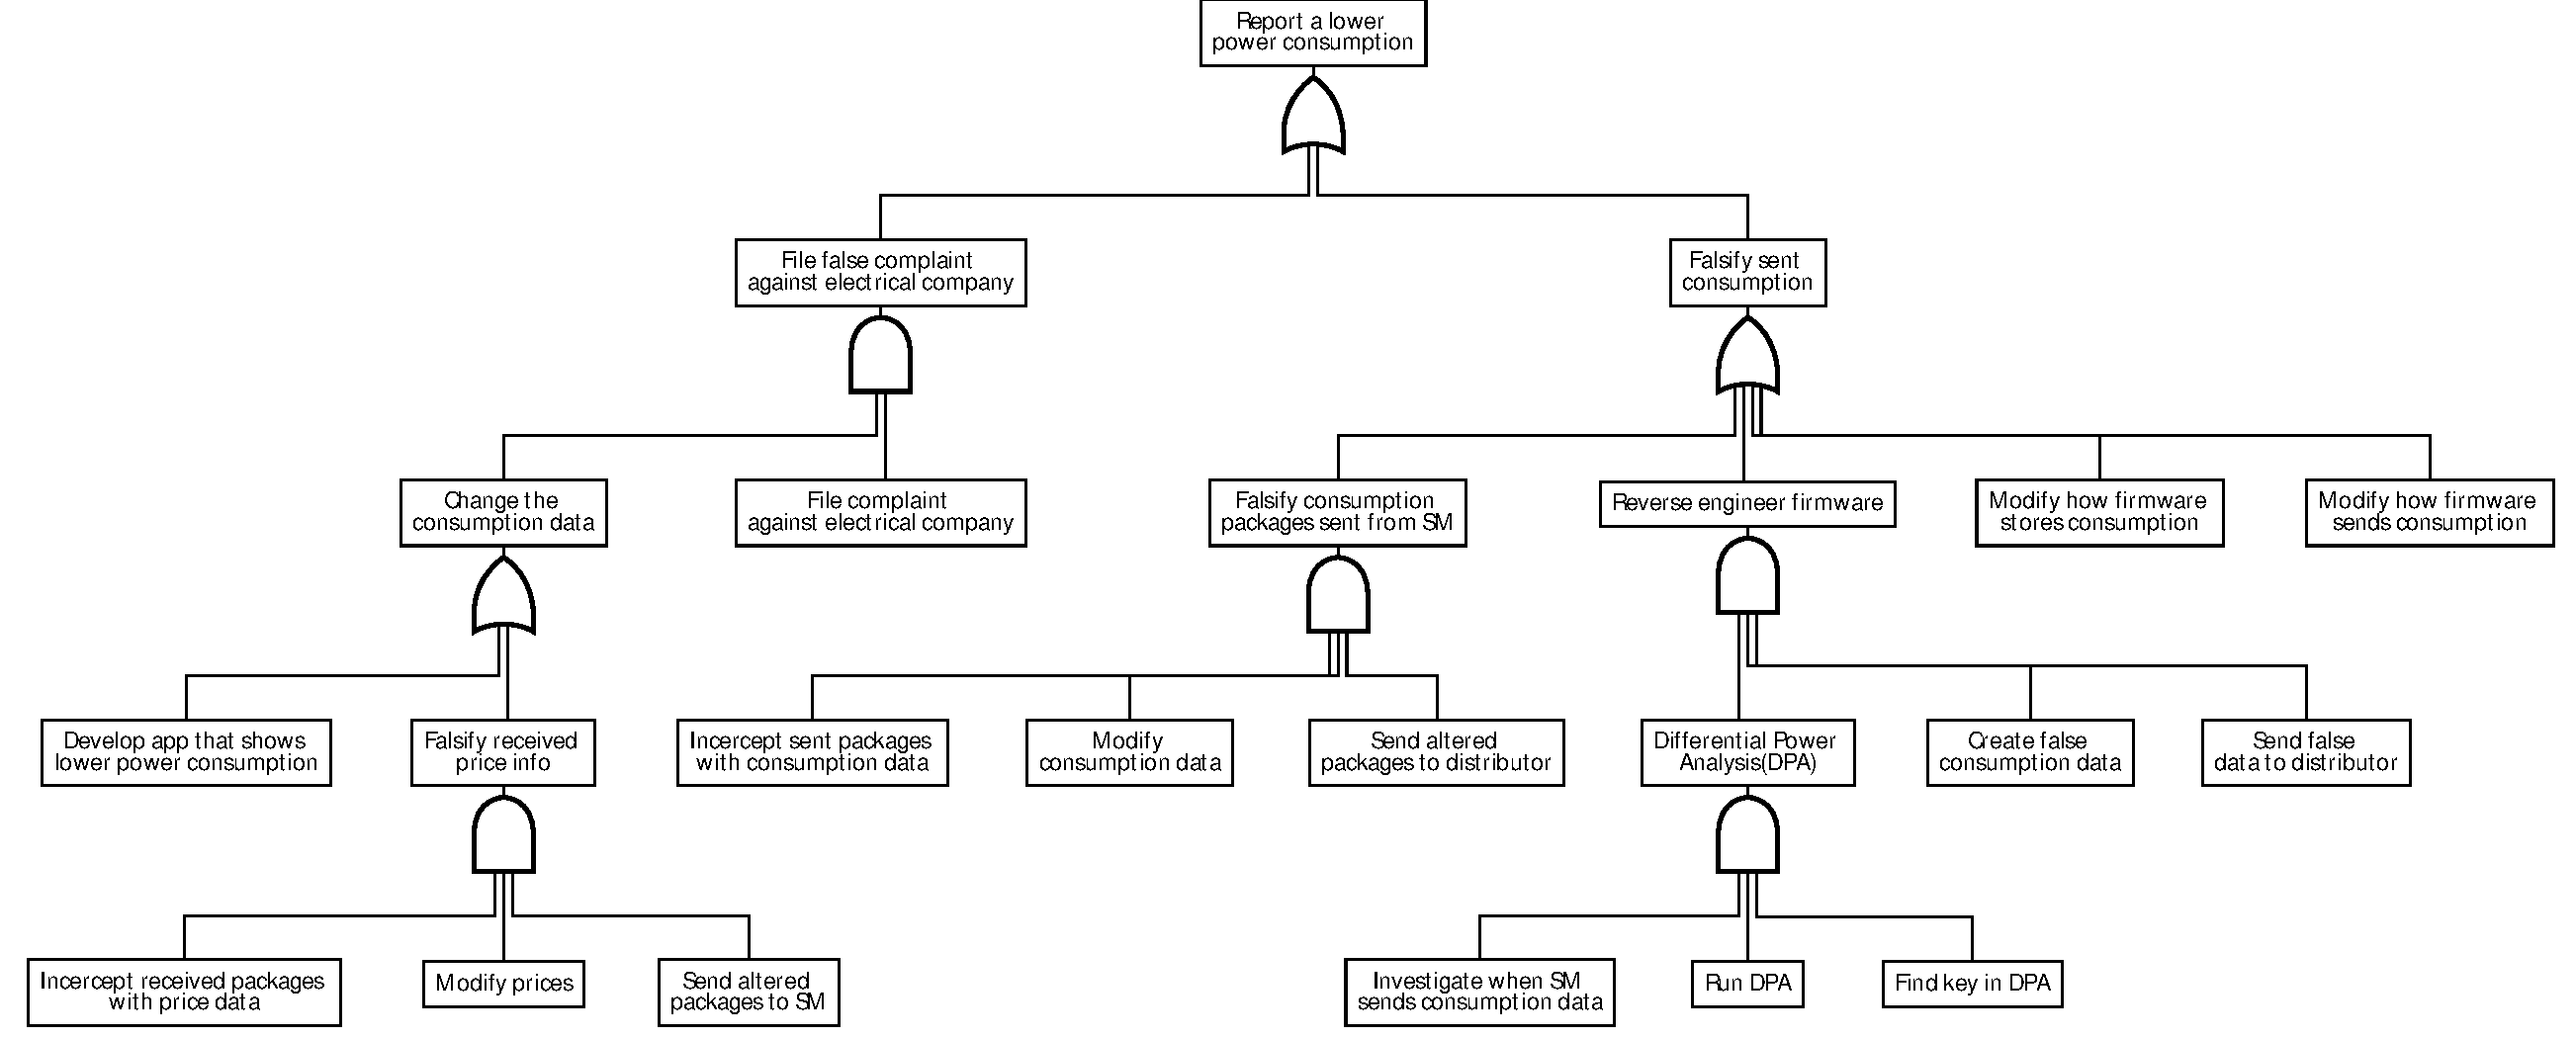
\includegraphics[width=1\textwidth]{graphics/consumer_orig.pdf}

\end{frame}

\begin{frame}{Consumer $\implies$ Electrical Company}
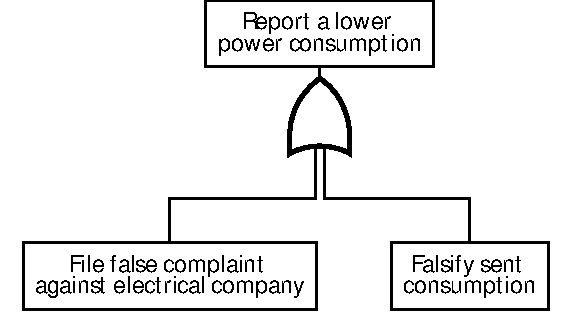
\includegraphics[width=1\textwidth]{graphics/consumer.pdf}

\end{frame}

\begin{frame}{Consumer $\impliedby$ Electrical Company}
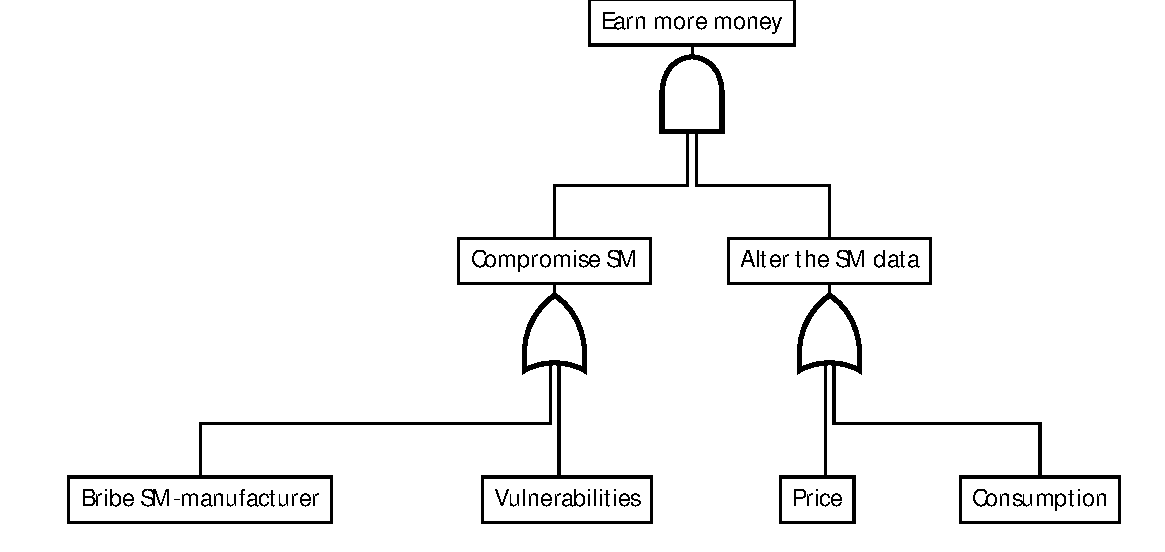
\includegraphics[width=\textwidth]{graphics/electrical_company_vs_consumer.pdf}

\end{frame}

\subsection*{Attacks from the vicinity}
\begin{frame}{Attacks from the vicinity}

\resizebox{!}{0.6\textwidth}
{
\tikzstyle{man}=[font={\Gentsroom}, scale=5]
\tikzstyle{woman}=[font={\Ladiesroom}, scale=5]

\begin{tikzpicture}[every node/.style={inner sep=0,outer sep=0}, arrows={[round]}]

\draw (-5.5,6) rectangle (2,-0.5);
\node at (-1,5.5) {Household};

\draw  (-6.5,7) [fill=white] rectangle (-4,5.5) node[pos=.5,align=center] {Home\\Production};
\draw  (-5,1.5) [fill=white] rectangle (-3.5,0) node[pos=.5,align=center] {Smart\\Meter};
\draw  (-3,4.5) [fill=white] rectangle (-1,3) node[pos=.5,align=center] {Smart\\Appliance};
\draw  (-0.5,2) [fill=white] rectangle (0.5,1) node[pos=.5,align=center] {Client};
\draw  (-9,2.5) [fill=white] rectangle (-6.5,1) node[pos=.5,align=center] {Data Hub};

\node[man] (consumer) at (1,1) {};
\node [below=0.2 of consumer] {Consumer};

\node[man] (burglar) at (-6.5,0) {};
\node [below=0.2 of burglar] {Burglar};

\node[man] (external) at (3.5,5) {};
\node [below=0.2 of external] {External};

\node[man] (power) at (-7.5,6.5) {};
\node [below=0.2 of power,align=center] {Electrical\\Company};

\node[man] (distribution) at (-7.5,4) {};
\node [below=0.2 of distribution] {Distribution};

\node[woman] (partner) at (1,4) {};
\node [below=0.2 of partner] {Partner};

\node[man] (neighbor) at (3.5,0.5) {};
\node [below=0.2 of neighbor] {Neighbor};

\draw[dashed] (-4.5,5.5) -- (-4.5,1.5);
\draw[dashed] (-6.5,1.5) -- (-6,1.5) -- (-6,1) -- (-5,1);
\draw[dashed] (-3.5,1) -- (-2.5,1) -- (-2.5,1.5) -- (-0.5,1.5);
\draw[dashed] (-2.5,3) -- (-2.5,2.25) -- (-4,2.25) -- (-4,1.5);


\draw<1>[ultra thick, red, -{Stealth[scale=1.2]}] (neighbor) -- (consumer);
\draw<1>[ultra thick, red, -{Stealth[scale=1.2]}] (partner) -- (consumer);
\draw<1>[ultra thick, red, -{Stealth[scale=1.2]}] (burglar) -- (consumer);

\draw<2>[ultra thick, red, -{Stealth[scale=1.2]}] (external) -- (consumer);


\end{tikzpicture}
}
\end{frame}

\begin{frame}{Attacks from the vicinity}
  Actors attacking the consumer have similar attack structure
\center
  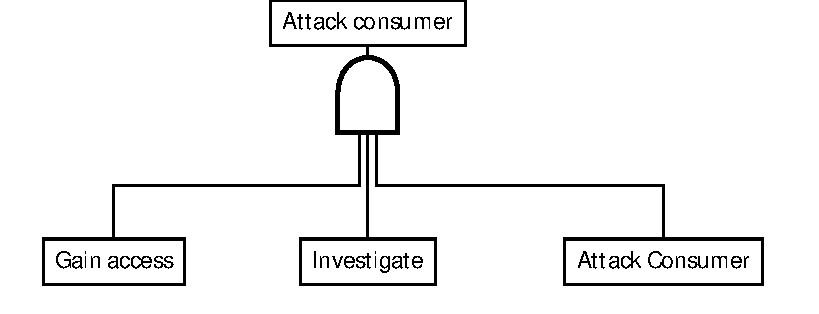
\includegraphics[width=0.7\textwidth]{graphics/common_attack.pdf}
\end{frame}

\begin{frame}{Gain access}
  \begin{block}{Accessing smart meter}
    \begin{itemize}
      \item Compromise Smart Meter
      \item Compromise Client
      \item Install ECM
    \end{itemize}
  \end{block}

  \begin{block}{Obtaining data }
    \begin{itemize}
      \item Buy power consumption data
      \item Obtain power consumption data
    \end{itemize}
  \end{block}
\end{frame}

\begin{frame}{Investigate}

\begin{tabular}{l l}

  
\includegraphics[width=0.4\textwidth]{graphics/hus.jpg}
&
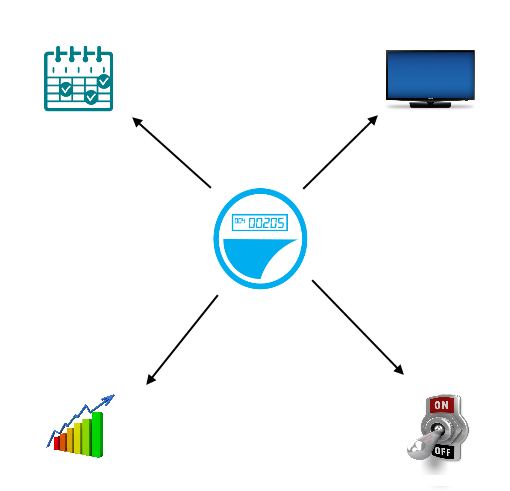
\includegraphics[width=0.4\textwidth]{graphics/smartmeterdata.png}
\end{tabular}

     \begin{itemize}
        \item When is the consumer home?
        \item What is the consumer doing?
        \item What does the consumer own?
        \item What behavioural patterns do the consumer practice?
      \end{itemize}
\end{frame}

\begin{frame}{Attack Consumer}
  \begin{columns}[T]
    \begin{column}{0.5\textwidth}
    \begin{block}{Direct attacks}
      Objective:
      \begin{itemize}
        \item Break in
        \item Remove annoyances
        \item Get revenge
      \end{itemize}
      Means:
      \begin{itemize}
        \item Control devices
        \item Change device schedules
      \end{itemize}
    \end{block}
\end{column}
\begin{column}{0.5\textwidth}
  \begin{block}{Indirect attacks}
    \begin{itemize}
      \item Create consumer profile
      \item Sell data
      \item Turn off power
    \end{itemize}
  \end{block}
\end{column}
\end{columns}
\end{frame}
